%% Einleitung.tex
%% $Id: einleitung.tex 61 2012-05-03 13:58:03Z bless $
%%

\chapter{Einleitung}
\label{ch:Einleitung}
%% ==============================
Während die Ortung im Außenbereich fest in der Hand von Satellitensystemen wie dem Global Positioning System (GPS) liegen, bietet die Ortung im Innenraum eine Vielzahl verschiedener Technologien. Neben Technologien wie Bluetooth, Radio Frequency Identification (RFID) und Ultra Wide Band (UWB) weckt WLAN wegen seiner großen Verbreitung immer wieder Interesse in Forschung und Industrie. \\
So hat die Ortung mittels WLAN gerade im medizinischen Bereich durch kommerzielle Lösungen Verbreitung gefunden, Probleme finden sich aber bei Ortungsgenauigkeit gegenüber anderen Techniken und dem vergleichsweise hohen Energieverbrauch des Protokolls.
Während viele wissenschaftliche Arbeiten sich der Ortungsgenauigkeit widmen, ist für den alltäglichen Einsatz die Batterielaufzeit der mobilen Einheiten hinderlich, wenn nicht gerade Smartphones als mobile Einheiten in Frage kommen. \\
Auch im Tunnelbau ist eine Ortung von Mitarbeitern und Besuchern von Nöten um in Notfällen bestimmen zu können, ob und wie viele Personen sich im Gefahrenbereich befinden, dies beeinflusst die Arbeit der Rettungskräfte. 
Das veränderliche Umfeld der Baustelle, auf der große Stahl- und Betonelemente bewegt werden, stellt dabei die genaue Ortung mittels Radiowellen vor große Probleme und es wird nur Bereichsortung durchgeführt, bei der jede Tunnelröhre in mehrere hundert Meter große Abschnitte aufgeteilt wird und der Wechsel der Mitarbeiter zwischen den Abschnitten beobachtet wird. 
Dies stellt zwar nur eine geringe Auflösung dar, erlaubt es aber bei Bränden zu erkennen welche Personen sich durch die Abschnitte Richtung Ausgang bewegen und welche in ihrem Abschnitt verharren, sie sind vermutlich entweder bewegungsunfähig oder eingeschlossen. 
Die geringe Auflösung hat zudem Vorteile bezüglich des Datenschutzes, da sie verhindert, dass die Arbeiter mit Bewegungsprofilen analysiert werden und zum Beispiel geprüft wird wer sich wie lange im Pausenraum aufhält.
Die Ortung wird derzeit bei einem Referenzunternehmen mittels Bluetooth durchgeführt, dabei sind die Knoten eigenständige Bluetooth Access Points, die mit dem Ethernet Backbone verbunden sind, als mobile Einheiten kommen sowohl batteriebetriebene Tags als auch Smartphones zum Einsatz. 
Das zentrale Sicherheitssystem fragt die gesehenen mobilen Einheiten bei den Knoten an und bereitet die Ergebnisse graphisch auf.
 
%% ==============================
\section{Zielsetzung der Arbeit}
%% ==============================
\label{ch:Einleitung:sec:Zielsetzung}
Ziel der Arbeit sollder Entwurf und die Implementierung eines Bereichsortungssystems für Personen in Tunnelanlagen unter Verwendung eines bestehenden Netzwerks von WLAN Access Points (APs) sein. 
Bei einem Bereichsortungssystem handelt es sich um ein Ortungssystem bei dem die Positionen nicht genau bestimmt werden. Stattdessen wird das Areal auf dem geortet werden soll in einzelne Bereiche unterteilt und jede mobile Einheit beim Vorgang des ortens einem dieser Bereiche zugeordnet.\\
Diese Arbeit grenzt sich von vorherigen Arbeiten dadurch ab, dass die Laufzeit beziehungsweise der Energieverbrauch der mobilen Einheiten im Vordergrund steht. 
Statt der nur wenige Tage umfassenden Laufzeiten anderer WLAN basierter Tags ist das Ziel dieser Arbeit eine Laufzeit von mehreren Monaten. \\
Der Entwurfsraum umfasst in einem ersten Schritt keine Änderungen an den Access Points, ihre Anzahl, Position, Software und Hardware ist gegeben. 
Anschließend wird diese Beschränkung gelockert und die Software der APs kann verändert werden, bei diesen Veränderungen sollen aber die grundlegenden Mechanismen der 802.11 Spezifikation erhalten bleiben. 
So soll es nicht assozierten Clients nicht möglich sein direkt mit Servern im Netzwerk zu kommunizieren, da dies die Sicherheit des gesamten Netzwerks gefährden könnte.
In einer zweiten Lockerung der Beschränkungen soll auch die Hardware veränderbar sein, dies widerspricht zwar der Annahme der bestehenden Struktur von WLAN APs, da diese potenziell ausgetauscht werden müssten, erweitert den Handlungsspielraum jedoch enorm und erlaubt es die vorherigen Implementierungen mit einer energetisch effizienten und potenziell nicht WLAN-basierten zu vergleichen. 
Für jeden dieser Schritte müssen die angrenzenden Komponenten, Ortungsserver und mobile Einheiten, implementiert und hinsichtlich des Energieverbrauchs und der Erkennungssicherheit evaluiert werden. Abschließend sollen die drei Systeme miteinander verglichen werden. \\


%% ==============================
\section{Anforderungen an das Bereichsortungssystem}
%% ==============================
\label{ch:Einleitung:sec:Anforderungen}
Da es sich um ein Bereichsortungssystem handeln soll werden keine direkten Anforderungen an die Genauigkeit der Ortung gestellt, jedoch soll ein klarer Wechsel zwischen zwei Bereichen, und damit zwei Access Points, zuverlässig erkannt werden. 
Bei den von den Zielpersonen getragenen Positionssendern, den sogenannten Tags, soll es in den ersten beiden Schritten um Geräte handeln, die auf WLAN Basis arbeiten und somit mit den Access Points kompatibel sind.
Im dritten Schritt ist dies nicht erforderlich und die Kompatibilität wird durch technische Änderungen am AP wiederhergestellt.
Die Tags sollen eine Laufzeit von bis zu 3 Jahren erreichen, sie müssen jedoch mindestens eine Laufzeit von 6 Monaten aufweisen um als verwendbar angesehen zu werden. 
Dabei sind Größe und Gewicht der Lösung zu beachten, zwar kann die Laufzeit eines Tags jederzeit durch die Vergrößerung des Energiespeichers herbeigeführt werden, die Tags müssen jedoch mühelos von den Zielpersonen an einem Band um den Hals getragen werden können.
Zuletzt soll unter Rücksichtnahme auf das beschriebene Szenario die Komplexität der IT-Infrastruktur so gering wie möglich gehalten werden um ein stabiles und kostengünstiges System zu garantieren. 

%% ==============================
\section{Klassifizierung von Ortungssystemen}
%% ==============================
\label{ch:Einleitung:sec:Ortungssysteme}
Die Klassifikation von Ortungssystemen auf Funkbasis kann neben dem verwendeten Protokoll anhand der Topologie, dem Lokalisationsprinzip und der gemessenen Größen durchgeführt werden \cite{liu2007survey}.
Außerdem wird zwischen zweidimensionaler und dreidimensionaler Lokalisation unterschieden.

\subsection{Protokoll}
Prinzipiell lassen sich verwendete Frequenzen, Modulationsverfahren und Sendeleistung frei wählen, solange sie die gesetzlichen Vorgaben für die Sender eingehalten werden. Wenn ein eigenes Protokoll verwendet wird kann die Kodierung der Informationen frei gewählt werden, ein Beispiel für ein solches Protokoll ist die Ortung mit Ultra-Breitband Signalen (UWB) mit dem Genauigkeiten im Zentimeterbereich erreicht werden können. Bestehende Protokolle zu verwenden hat dagegen den Vorteil, dass üblicherweise commodity-of-the-shelf Komponenten verwendet werden können, was die Kosten des Systems senkt. Im Gegenzug können für die Genauigkeit wichtige Parameter nicht mehr frei gewählt werden und der overhead des Protokolls muss übernommen werden, Beispiele für solche Protokolle sind 802.11 (WLAN), Bluetooth und Radio Frequency Identification (RFID).

\subsection{Topologie}
Die Topologie hat zwei Dimensionen, Fernlokalisation versus Selbstlokalisation und direkt versus indirekt und beschreibt wie Knoten und mobile Einheiten zusammenwirken. \\
Bei der direkten Fernlokalisation werden von mobilen Einheiten gesendete Signale an Knotenpunkten gemessen und die Ergebnisse an einen zentralen Ortungsserver weitergegeben, dieser führt dann die Lokalisation durch. Das Ergebnis der Lokalisation ist nur zentral verfügbar. \\
Bei der direkten Selbstlokalisation senden hingegen die Knoten und die mobilen Einheiten messen die eingehenden Signale. Anhand der Messergebnisse bestimmt jede mobile Einheit seine Position, die Ergebnisse der Lokalisation sind anschließend nur auf der mobilen Einheit verfügbar. \\
Die indirekte Fernlokalisation gleicht der direkten Selbstlokalisation, allerdings besteht zusätzlich eine Datenverbindung zu einem zentralen Ortungsserver, dem die berechnete Position mitgeteilt wird. Das Ergebnis steht nach kurzer Verzögerung sowohl auf der mobilen Einheit als auch zentral zur Verfügung, optional können dort die Daten von anderen mobilen Einheiten zugegriffen werden um sich über deren Positionen zu informieren. \\
Auch die indirekte Selbstlokalisation erweitert die direkte Fernlokalisation um eine Datenverbindung zum zentralen Ortungsserver, um sich über die eigene und eventuelle auch andere mobile Einheiten zu informieren. Dies kann insbesondere bei Verwendung von Mischtechnologien notwendig sein, wenn die zur Ortung genutzte Technik es nicht erlaubt an den mobilen Einheiten zu empfangen, aber dennoch eine Selbstlokalisation durchgeführt werden soll.

\subsection{Lokalisationsprinzip}
Das einfachste Lokalisationsprinzip ist das Umgebungsprinzip, hier wird eine mobile Einheit dem Knoten mit dem stärksten Signal zugeordnet, der Knoten kann sowohl als Sender als auch als Empfänger auftreten. Die gewonnene Position ist dabei nur symbolisch und ihre Genauigkeit ist abhängig von der Dichte des Netzes. Für eine erfolgreiche Lokalisation muss nur ein Knoten in Reichweite der mobilen Einheit sein, was diese Möglichkeit auch in komplexeren Lokalisationsprinzipien zu einer sinnvollen Ausweichmöglichkeit macht, falls nicht genügend Knoten in Reichweite sind. \\
Die geometrische Bestimmung der Position einer mobilen Einheit mit drei Knoten nennt man Trilateration. Dabei wird üblicherweise für jeden Knoten die Distanz zur mobilen Einheit bestimmt, anschließend wird ein Kreis mit der gemessenen Distanz um jeden Knoten gebildet und der Schnittpunkt der drei Kreise bestimmt die Position der mobilen Einheit. Da die Distanzen aus den gemessenen Signalparametern geschätzt werden müssen sind sie fehlerbehaftet und es ergibt sich oft kein eindeutiger Schnittpunkt, dann wird zum Beispiel die Mitte der existierenden Schnittpunkte gewählt. \\
Die geometrische Bestimmung ist ebenfalls über die Berechnung der Winkel zu den Knoten möglich, dies nennt man Triangulation. Der Winkel kann zum Beispiel über die zeitlich Differenz der ankommenden Signale an den synchronisierten Knoten bestimmt werden, dann wird von jedem Knoten aus eine Halbgerade in diesem Winkel gefällt und der Schnittpunkt bestimmt die Position der mobilen Einheit. Wenn mit gerichteten Antennen gearbeitet wird kann der Winkel des eingehenden Signals direkt bestimmt werden, dann müssen nur 2 Knoten in Reichweite sein um die mobile Einheit zu lokalisieren. \\
Das aufwendigste Lokalisationsprinzip ist die Szenenanalyse. Hier werden zunächst in einer offline-Phase Vektoren $(m_1,m_2,...,m_n,p_x,p_y,p_z)^T$ aus Messgrößen und Positionsmarken gesammelt, anhand dieser Fingerabdrücke werden dann in der online-Phase die Positionen neuer Messergebnisse bestimmt. Üblicherweise kommen dabei Verfahren des maschinellen Lernens wie k-nearest-neighbour, neuronale Netze oder Support Vektor Machines (SVM) zum Einsatz um die Muster der Fingerabdrücke aus der offline-Phase zu erkennen und die Positionen $(p_x,p_y,p_z)^T$ in der online-phase aus den gemessenen Größen $(m_1,m_2,...,m_n)^T$ zu schätzen. Im zweidimensionalen Fall wird dabei $p_z = 0$ angenommen.

\subsection{Messgrößen}
Beliebte Messgrößen für die Positionsbestimmung sind Ankunftszeit des Signals (time of arrival, TOA), die Differenz der Ankuftszeiten (time difference of arrival, TDOA), die Paketumlaufzeit (roundtrip time of flight, RTOF) und die Stärke des empfangenen Signals (received signal strength, RSS). Es existieren aber noch mehr messbare Größen, wie etwa die Messung der empfangenen Phase des Signals (received signal phase, RSP) und die Messung des Einfallsswinkel des Signals mit mehreren gerichteten Antennen (angle of arrival, AOA). \\
%TODO Muss man nicht c in s/m angebeben?
TOA beruht auf der begrenzten Ausbreitungsgeschwindigkeit des Signals, hochfrequente Signale breiten sich mit Lichtgeschwindigkeit $c = 299.792.458m/s$, Ultraschall mit Schallgeschwindigkeit $c \approx 343m/s$ bei $20^{\circ}C$, aus, damit ergibt sich die Distanz $d = \frac{t_{empfangen,i} - t_{gesendet}}{c}$ mit $i$ sei der empfangende Knoten. Die Position der mobilen Einheit kann dann mit der Methode der kleinsten Quadrate bestimmt werden, dazu wird die Kostenfunktion $F(x,y,t) = \sum_{i=1}^{N} {\alpha}^2_i f^2_i(x,y,t)$ mit $f_i(x,y,t) = c(t_i - t) - \sqrt{(x_i - x)^2 + (y_i - y)^2}$ und ${\alpha}_i$ sei die Konfidenz von Knoten $i$, minimiert. Dies erfordert, dass die Knoten synchronisiert sind und die $t_i$ möglichst ohne vorherige Verarbeitung bestimmt wird um Varianzen zu vermeiden. Zusätzlich ist es von Vorteil, wenn auch die mobile Einheit synchronisiert ist, da dann nur noch mit zwei Variablen optimiert werden muss, da $t$ dann entsprechend der Synchronisation und dem Sendeintervall als gegeben angenommen werden kann. Die Forderung nach Synchronität ist jedoch für $c = 299.792.458m/s$ sehr stark, da das Signal nur $0.00000000336 s/m$ benötigt und somit bereits kleine zeitliche Ungenauigkeiten große Fehler verursachen und erst durch zusätzliche Messungen oder Glättungstechniken hohe Genauigkeiten erreicht werden können. Skibniewski et al. konnten hohe Genauigkeit durch die Verwendung von Ultraschall erzielen, da sich durch die geringere Ausbreitungsgeschwindigkeit Imperfektionen in der Synchronisierung weniger stark auswirken \cite{skibniewski2009simulation}. 
Bei einer Selbstlokalisation ist zu beachten, dass $t$ den Sendezeitpunkt der Knoten darstellt, sie müssen also entweder alle gleichzeitig auf verschiedenen Frequenzen oder in einem vordefinierten Muster nacheinander senden, die Zeitdifferenz des tatsächlichen Sendezeitpunkts zu $t$ muss dann vom Empfangszeitpunkt $t_i$ abgezogen werden. \\
Bei TDOA wird statt der direkten Ankunftszeiten die Differenz dieser gemessen, dies erfordert üblicherweise Zeitsynchronität bei den Knoten, nicht jedoch bei der mobilen Einheit, da nur die Ankuftszeiten für die Berechnung relevant sind. Die mobile Einheit liegt dabei auf auf dem Schnittpunkt zweier Hyperboloiden, die jeweils zwischen den Knoten die TDOA gemessen haben und einem Referenzknoten aufgespannt werden. 
Die Hyperboloiden werden aufgestellt durch \\
$R_{i,j} = \sqrt{(x_i - x)^2 + (y_i - y)^2 + (z_i - z)^2} - \sqrt{(x_i - x)^2 + (y_i - y)^2 + (z_i - z)^2}$ mit $(x_i,y_i,z_i)$ sei der jeweilige Messknoten, $(x_j,y_j,z_j)$ sei der gemeinsame Referenzknoten und $(x,y,z)$ sei die Position der mobile Einheit. Abb. \ref{fig:tdoa} zeigt die Lösung graphisch, Drane et. al. und Torrieri beschreiben die analytische Lösung der Gleichung mit nichtlinearer Regression \cite{drane1998positioning} beziehungsweise Taylor-Entwicklung \cite{torrieri1984statistical}. 
Li et al. eliminiert zusätzlich die Forderung nach Synchronisation für mobile Einheiten, die sowohl senden als auch empfangen können \cite{li2000comparison}. 
Dabei wird ein Datenpaket an die mobile Station gesendet und von dieser mit einem Acknowledgement beantwortet, diese Kommunikation wird von anderen Knoten beobachtet und die Differenz der Ankunftszeiten des Datenpakets und des Acknowledgements als $t_{i,1}$ mit $i \in Knoten$ protokolliert. Zusätzlich ist $t_{i,0}$ als die Differenz zwischen dem Senden des Datenpakets und dem Empfangen an den anderen Knoten durch die bekannte Position aller Knoten ebenfalls bekannt. Damit kann die Differenz der Ankunftszeit $TDOA_{i,j} = (t_{i,0} + t_{i,1}) - (t_{j,0} + t_{j,1})$ mit $i,j \in Knoten$ ohne vorherige Synchronisation berechnet werden. \\
Wird RTOF gemessen muss die mobile Einheit sowohl senden als auch empfangen können. Dabei wird die Zeit vom Aussenden eines Paketes bis zur Ankunft der Antwort gemessen, wichtig sind hier zum einen möglichst spät/früh gesetzten Zeitstempel beim senden/empfangen des Signals und eine sehr konstante Verarbeitungszeit des Kommunikationspartners. Zunächst muss dabei die Verarbeitungszeit gemessen werden, indem Knoten und mobile Einheit auf einen Abstand von 0 Metern gebracht werden, anschließend kann die Entfernung $d = \frac{t_{empfangen} - t_{gesendet} - t_{Verarbeitung}}{c}$ bestimmt werden. Die Position wird dann analog zu TOA bestimmt. Diese Messgröße kann sowohl für die Fern- als auch für die Selbstlokalisation verwendet werden, ist aber sehr anfällig gegenüber Schwankungen in der Verarbeitungszeit, die bei Protokollen wie 802.11 häufig auftreten. \\
RSS überprüft wie stark das empfangene Signal aus dem allgemeinen Rauschen auf der verwendeten Frequenz hervor sticht. Dafür ist es wichtig, dass immer mit der selben Leistung gesendet wird, dann kann mit einem theoretisch oder empirisch ermittelten Ausbreitungsmodell die Entfernung zwischen mobiler Einheit und Knoten anhand des Pfadverlustes bestimmt werden. Dann ist $d = F(S_{gesendet},S_{empfangen})$ mit $F$ sei das Ausbreitungsmodell. Um gute Ergebnisse zu erzielen sollten jeweils möglichst gleichförmige mobile Einheiten und Knoten verwendet werden, denn Lui et al. konnte für WLAN zeigen, dass unterschiedliche Hardware bei Knoten und mobiler Einheit erhebliche Varianz in den gemessenen RSS Werten erzeugt \cite{lui2011differences}. Zusätzliche Probleme entstehen, wenn Protokolle wie Bluetooth eine Anpassung der Sendeleistung vorsehen \cite{hossain2007comprehensive}, dann muss eine solche Anpassung eliminiert werden, bei Bluetooth geschiet das durch die Verwendung von \textit{Inquiry} Paketen, diese dienen zur Entdeckung anderer Bluetooth-fähiger Geräte und werden immer mit voller Sendeleistung gesendet um möglichst alle Geräte in Reichweite zu erreichen.
Ein weiteres Problem von RSS ist der starke Einfluss von Hindernissen und anderen  Signalen auf dem selben Frequenzband. Gerade bei der Ortung in Innenräumen wirken diese Einflüsse begrenzend auf die Genauigkeit und oft muss eine Kalibrierung durchgeführt werden um die Einflüsse von Wänden und anderen Hindernissen zu eliminieren.

\begin{figure}[!htbp]
  \centering
	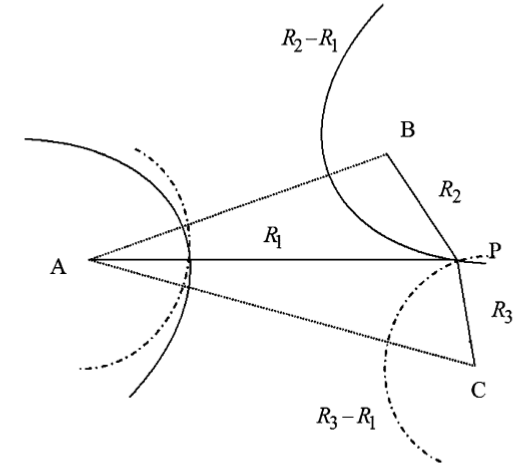
\includegraphics[width=0.5\textwidth]{images/tdoa.png}
  \caption{Positionsbestimmung mit der Differenz der Ankunftszeiten (TDOA), aus \cite{liu2007survey}.}
  \label{fig:tdoa}
\end{figure}

%% ==============================
\section{Gliederung der Arbeit}
%% ==============================
\label{ch:Einleitung:sec:Gliederung}
Im folgenden Kapitel 2 sollen zunächst einige wissenschaftliche und kommerzielle Lösungen zur Ortung in Innenräumen diskutiert werden. 
Anschließend wird in Kapitel 3 die Spezifikation 802.11, auch wireless LAN (WLAN) genannt, in einem für diese Arbeit notwendigem Maße erörtert. Dort werden auch die für das Ortungssystem nötigen Teile der Bluetooth 4.0 (Low Energy) Spezifikation erläutert. 
In Kapitel 4 wird eine Übersicht über die Hardware der Bluetooth und WLAN Tags und deren Programmiermöglichkeiten gegeben. 
Im Anschluss wird in Kapitel 5 der Entwurfsraum im Rahmen einer theoretischen Betrachtung abgesteckt. 
Die nachfolgenden Kapitel 6 und 7 widmen sich der Methodik und Ausführung von Experimenten bezüglich Energieverbrauch und Reichweite der Tags.
Die Implementierung der Ortungsserver und die Schnittstellen zu Access Points und Sicherheitssystem werden in Kapitel 8 beschrieben.
Zum Schluss folgt ein Fazit, welches die Ergebnisse zusammenfasst und die evaluierten Lösungsansätze abschließend vergleicht.

%%% Local Variables: 
%%% mode: latex
%%% TeX-master: "thesis"
%%% End: 
